\documentclass[conference]{IEEEtran}
\IEEEoverridecommandlockouts

\usepackage{cite}
\usepackage{amsmath,amssymb,amsfonts}
\usepackage{algorithmic}
\usepackage{graphicx}
\usepackage{textcomp}
\usepackage{xcolor}
\usepackage{booktabs}
\usepackage{array}
\usepackage{listings}
\usepackage{courier}
\usepackage{enumitem}
\usepackage{verbatim}
\usepackage{multirow}
\usepackage{hyperref}
\usepackage{fancyhdr}

\hypersetup{
    colorlinks=true,
    linkcolor=blue,
    filecolor=blue,      
    urlcolor=blue,
    citecolor=blue,
}

% Listings configuration for Python code blocks
\lstset{
    basicstyle=\footnotesize\ttfamily,
    breaklines=true,
    breakatwhitespace=true,
    showstringspaces=false,
    frame=single,
    columns=fullflexible,
    numbers=none,
    keywordstyle=\color{blue}\bfseries,
    commentstyle=\color{gray},
    stringstyle=\color{teal},
    language=Python
}

% Configure footer
\pagestyle{fancy}
\fancyhf{}
\fancyfoot[C]{Makalah IF2123 Aljabar Linear dan Geometri -- Semester 1 Tahun 2025/2026}
\renewcommand{\headrulewidth}{0pt}
\renewcommand{\footrulewidth}{0pt}

% Ensure first page also uses the same footer
\fancypagestyle{plain}{%
  \fancyhf{}
  \fancyfoot[C]{Makalah IF2123 Aljabar Linear dan Geometri -- Semester 1 Tahun 2025/2026}
  \renewcommand{\headrulewidth}{0pt}
  \renewcommand{\footrulewidth}{0pt}
}

\begin{document}

\title{Penerapan Eigenvalue Decomposition dan Power Iteration Method dalam Analisis Kerentanan Jaringan Drainase Perkotaan}

\author{
    \IEEEauthorblockN{
        Nashiruddin Akram - 13524090\textsuperscript{1}
    }
    \IEEEauthorblockA{
        \textit{Program Studi Teknik Informatika} \\
        \textit{Sekolah Teknik Elektro dan Informatika} \\
        \textit{Institut Teknologi Bandung, Jl. Ganesha 10 Bandung 40132, Indonesia} \\
        \textsuperscript{1}\textit{\href{mailto:akrambaasir@gmail.com}{akrambaasir@gmail.com}}, \textit{\href{mailto:13524090@std.stei.itb.ac.id}{13524090@std.stei.itb.ac.id}}
    }
}

\maketitle
\thispagestyle{fancy}

\begin{abstract}
Jaringan drainase perkotaan adalah salah satu elemen penting dalam mencegah banjir, namun cara analisisnya saat ini masih terbatas---hanya memeriksa komponen per komponen tanpa melihat bagaimana semua bagian terhubung dan saling memengaruhi. Makalah ini mengusulkan pendekatan baru menggunakan aljabar linear, khususnya eigenvalue decomposition dan power iteration method, untuk menemukan titik-titik kritis dalam jaringan drainase yang dimodelkan sebagai matriks Laplacian. Dengan menggabungkan analisis topologi jaringan (spectral centrality) dan parameter fisik seperti elevasi, kapasitas aliran, serta sedimentasi, penulis menganalisis jaringan drainase dummy dengan 200 nodes dan 851 edges. Hasil menunjukkan algebraic connectivity $\lambda_2 = 0.075$ mengindikasikan jaringan sangat rentan terhadap pemisahan. Sekitar 30\% titik termasuk kategori kerentanan tinggi, dan korelasi eigenvalue centrality terhadap vulnerability mencapai $r = 0.715$, membuktikan metode ini efektif untuk menilai kerentanan sistem. Analisis sensitivitas bobot menunjukkan model robust terhadap variasi parameter moderat (Jaccard index $\approx$ 1.0 di sekitar konfigurasi baseline), dan partisi spektral berhasil membagi jaringan menjadi zona pemeliharaan yang koheren. Metode ini dapat digunakan untuk memprioritaskan pemeliharaan preventif dan mengembangkan sistem monitoring berbasis waktu nyata.
\end{abstract}

\begin{IEEEkeywords}
matriks Laplacian, eigenvalue decomposition, power iteration method, spectral centrality, jaringan drainase, analisis kerentanan
\end{IEEEkeywords}

\section{PENDAHULUAN}

\begin{figure}[h]
    \centering
    \includegraphics[width=0.38\textwidth]{Drainase.png}
    \caption{Ilustrasi Drainase}
\end{figure}

Sistem drainase perkotaan punya peran yang sangat penting dalam mencegah banjir dan mengelola air permukaan di area perkotaan. Sayangnya, pertumbuhan kota yang cepat telah banyak mengubah cara air mengalir—semakin banyak jalanan aspal dan bangunan beton, semakin sedikit tanah yang bisa menyerap air, dan aliran air pun berubah. Akibatnya, volume air hujan yang harus ditampung sistem drainase terus meningkat, sementara kapasitas saluran drainase yang ada tidak mengalami penambahan. Ditambah dengan curah hujan yang semakin sering dan lebat karena perubahan iklim, risiko banjir di kota-kota besar menjadi semakin mengkhawatirkan. Salah satu contoh nyata adalah banjir yang sering terjadi di Jakarta, di mana kegagalan sistem drainase akibat saluran tersumbat atau tidak terawat menyebabkan genangan air yang melumpuhkan aktivitas kota. Insiden seperti ini menunjukkan pentingnya analisis sistemik terhadap jaringan drainase—bukan hanya melihat kapasitas per saluran, tapi juga bagaimana semua sistem drainase saling terhubung dan pengaruhnya satu sama lain.

Cara konvensional yang biasa dipakai untuk mengecek kondisi drainase biasanya cuma fokus pada hal-hal yang sifatnya lokal: ukuran saluran, berapa banyak endapan lumpur yang numpuk, atau kondisi fisik setiap komponen. Memang cara ini berguna untuk perawatan rutin, namun ada kelemahannya—metode ini tidak dapat menangkap efek berantai yang terjadi apabila satu titik penting rusak atau macet. Misalnya, jika saluran utama di persimpangan penting tersumbat, air dapat meluap dan membanjiri area sekitarnya yang bergantung pada saluran tersebut, sementara saluran-saluran lain masih berfungsi normal. Inilah yang mendorong penulis mencoba pendekatan lain: menggunakan teori graf untuk melihat jaringan drainase secara keseluruhan. Lewat analisis spektral pada matriks Laplacian, kita bisa menemukan titik-titik mana yang paling kritis buat stabilitas seluruh sistem.

Matriks Laplacian adalah salah satu cara merepresentasikan struktur jaringan dalam bentuk matematis. Konsep ini mungkin terdengar abstrak, tapi sebenarnya cukup intuitif: dengan mengubah jaringan drainase menjadi matriks (tabel angka-angka), kita bisa menggunakan alat matematika yang powerful untuk menganalisisnya. Melalui eigenvalue decomposition (dekomposisi nilai eigen), kita bisa menganalisis seberapa kuat konektivitas jaringan dan seberapa mudah jaringan ini "pecah" kalau ada gangguan. Nilai eigen kedua terkecil ($\lambda_2$), yang sering disebut algebraic connectivity, memberikan informasi tentang seberapa robust jaringan terhadap fragmentasi --- semakin kecil nilainya, semakin rentan jaringan terhadap pemisahan. Selain itu, eigenvector dominan dari matriks adjacency—yang dapat dihitung secara efisien dengan power iteration method—menunjukkan titik mana yang paling berpengaruh dalam jaringan. Dalam makalah ini, penulis menggabungkan kedua metode aljabar linear tersebut dengan data fisik seperti elevasi, kapasitas aliran, risiko sedimentasi, dan beban hidraulik untuk membuat ranking titik-titik kritis yang dapat menjadi prioritas pemeliharaan.



\section{DASAR TEORI}

\subsection{Graf dan Matriks Adjacency}
Graf $G = (V, E)$ adalah struktur matematis yang terdiri dari himpunan simpul $V$ (titik-titik) dan himpunan sisi $E$ (penghubung antar titik). Dalam konteks jaringan drainase, simpul mewakili titik pertemuan atau percabangan saluran, sedangkan sisi merepresentasikan konektivitas antar saluran.

Matriks adjacency $A$ berukuran $n \times n$ merepresentasikan hubungan konektivitas:
\[
A_{ij} =
\begin{cases}
1, & \text{jika simpul } i \text{ dan } j \text{ terhubung}, \\
0, & \text{jika tidak terhubung}.
\end{cases}
\]

\subsection{Nilai Eigen dan Vektor Eigen}
Untuk matriks persegi $A$, nilai eigen $\lambda$ dan vektor eigen $x$ adalah konsep penting dalam aljabar linear yang didefinisikan lewat persamaan:
\[
A x = \lambda x.
\]
Secara intuitif, vektor eigen adalah vektor yang arahnya tidak berubah ketika dikalikan dengan matriks $A$ --- hanya panjangnya yang berubah, dan perubahan panjang tersebut ditentukan oleh nilai eigen $\lambda$. Dalam konteks jaringan, vektor eigen dominan menunjukkan pola pengaruh atau "aliran kepentingan" yang paling kuat dalam sistem.

Nilai eigen bisa dicari dengan menyelesaikan:
\[
\det(A - \lambda I) = 0.
\]

Vektor eigen yang sesuai dengan nilai eigen terbesar punya arti penting dalam analisis jaringan, terutama untuk mengukur seberapa besar pengaruh suatu simpul terhadap sistem keseluruhan.

\subsection{Eigenvalue Centrality}
Eigenvalue centrality mengukur tingkat kepentingan sebuah simpul berdasarkan seberapa banyak dia terhubung dengan simpul-simpul lain yang juga penting.

Jika $c_i$ adalah skor sentralitas simpul $i$, maka:
\[
c_i = \frac{1}{\lambda} \sum_{j=1}^{n} A_{ij} c_j.
\]
Dalam bentuk matriks, sentralitas memenuhi:
\[
A c = \lambda c,
\]
di mana $c$ adalah vektor eigen dari $A$ yang sesuai dengan nilai eigen terbesar $\lambda$.

Jadi, eigenvalue centrality ini memberi tahu kita simpul mana yang paling "sentral" atau paling berpengaruh dalam jaringan.

\subsection{Power Iteration}
Power iteration adalah metode numerik sederhana tapi efektif untuk menghitung nilai eigen terbesar dan vektor eigennya. Metode ini bekerja dengan cara yang intuitif: kita mulai dengan vektor sembarang, kemudian berulang kali mengalikannya dengan matriks dan menormalisasi hasilnya. Setelah beberapa iterasi, vektor ini akan "konvergen" atau mendekati eigenvector dominan. Karena matriks adjacency pada jaringan drainase bisa sangat besar (ratusan atau ribuan simpul), metode ini jadi sangat berguna karena efisiensinya.

Algoritma dasarnya cukup simpel:
\[
x^{(k+1)} = \frac{A x^{(k)}}{\| A x^{(k)} \|}.
\]
Normalisasi dengan membagi $\|A x^{(k)}\|$ dilakukan untuk mencegah overflow numerik dan menjaga panjang vektor tetap 1.

Kita iterasi terus sampai vektor $x$ konvergen ke vektor eigen dominan, dengan syarat matriks punya nilai eigen terbesar yang unik dan lebih besar secara absolut dari nilai eigen lainnya ($|\lambda_1| > |\lambda_i|$ untuk $i \neq 1$). Untuk matriks adjacency jaringan terhubung yang non-negatif, syarat ini umumnya terpenuhi berdasarkan teorema Perron-Frobenius.

\subsection{Spectral Radius}
Spectral radius $\rho(A)$ didefinisikan sebagai nilai absolut terbesar dari semua nilai eigen matriks adjacency:
\[
\rho(A) = \max_i |\lambda_i|.
\]
Spectral radius memberikan informasi tentang seberapa "kuat" koneksi dalam jaringan dan seberapa cepat informasi atau pengaruh bisa menyebar. Nilai yang tinggi mengindikasikan adanya hub nodes (simpul pusat) yang sangat dominan dalam jaringan.

Dalam konteks jaringan drainase, spectral radius bisa kasih info tentang:
\begin{itemize}
    \item seberapa stabil aliran air dalam jaringan,
    \item seberapa sensitif jaringan terhadap perubahan struktur,
    \item potensi titik rawan saat terjadi peningkatan debit air.
\end{itemize}

\subsection{Matriks Laplacian}
Matriks Laplacian $L$ adalah representasi alternatif dari graf yang menangkap informasi struktural lebih lengkap dibanding matriks adjacency. Matriks ini menggabungkan informasi tentang koneksi antar simpul (dari matriks adjacency) dengan informasi tentang berapa banyak koneksi yang dimiliki setiap simpul (dari matriks degree). Untuk graf dengan matriks adjacency $A$ dan matriks derajat $D$ (diagonal dengan $D_{ii} = \sum_j A_{ij}$), matriks Laplacian didefinisikan sebagai:
\[
L = D - A.
\]

Matriks Laplacian memiliki sifat-sifat penting:
\begin{itemize}
    \item Simetris dan semi-definit positif
    \item Nilai eigen terkecil selalu $\lambda_1 = 0$ dengan vektor eigen konstan
    \item Nilai eigen kedua terkecil $\lambda_2$ (disebut \textit{algebraic connectivity}) mengukur seberapa kuat graf terhubung
\end{itemize}

Nilai $\lambda_2$ yang kecil mengindikasikan graf mudah terpecah menjadi komponen terpisah, sedangkan $\lambda_2$ yang besar menunjukkan konektivitas yang robust.

\subsection{Normalized Laplacian}
Untuk dataset dengan distribusi degree yang tidak merata, normalized Laplacian memberikan hasil analisis spektral yang lebih stabil:
\[
\mathcal{L} = D^{-1/2} L D^{-1/2} = I - D^{-1/2} A D^{-1/2}.
\]

Normalized Laplacian memiliki spektrum nilai eigen dalam rentang $[0, 2]$ dan mengurangi bias dari simpul dengan degree ekstrem. Bentuk ini sangat berguna untuk jaringan drainase di mana terdapat hub dengan banyak koneksi dan simpul peripheral dengan koneksi sedikit.

\subsection{Fiedler Vector}
Vektor eigen yang bersesuaian dengan $\lambda_2$ dari matriks Laplacian (atau normalized Laplacian) disebut \textit{Fiedler vector}. Vektor ini memiliki interpretasi khusus dalam analisis jaringan:
\begin{itemize}
    \item Komponen vektor dengan tanda berbeda mengindikasikan partisi alami graf
    \item Simpul dengan nilai absolut besar dalam Fiedler vector adalah simpul yang paling sensitif terhadap pemisahan jaringan
    \item Dapat digunakan untuk spectral clustering dan identifikasi zona kerentanan
\end{itemize}

Dalam praktiknya, Fiedler vector dari normalized Laplacian lebih sering digunakan karena memberikan hasil yang lebih stabil untuk graf dengan distribusi degree heterogen.



\section{METODOLOGI PENELITIAN}

Berdasarkan dasar teori yang telah dipaparkan, metodologi penelitian ini dirancang untuk melakukan analisis spektral pada jaringan drainase dummy dengan 200 titik sebagai prototype. Penggunaan data dummy dipilih karena data riil jaringan drainase perkotaan yang lengkap dan terstruktur (mencakup topologi jaringan, parameter hidraulik, dan metadata simpul) sangat sulit diakses secara publik karena alasan keterbatasan dokumentasi. Dataset dummy yang digunakan dirancang untuk merepresentasikan karakteristik realistis jaringan drainase perkotaan berdasarkan literatur dan standar teknis yang ada. Pendekatan berbasis matriks Laplacian digunakan untuk menemukan simpul-simpul yang paling rentan, sehingga metodologi yang dikembangkan dapat diterapkan pada data riil di masa mendatang. Metodologi ini dibagi menjadi lima tahap utama yang saling terkait.

\subsection{Tahap I: Pemodelan Graf Jaringan Drainase}

Tahap pertama ini fokus pada pembangunan model matematis jaringan drainase dalam bentuk graf berarah $G = (V, E)$, di mana setiap simpul mewakili titik saluran atau percabangan, dan setiap sisi mewakili arah aliran air.

\bigskip
\subsubsection{Konstruksi Dataset dan Graf}
Dataset jaringan drainase disusun menjadi himpunan simpul $V$ dan sisi $E$ yang merepresentasikan struktur konektivitas. Dataset yang digunakan penulis terdiri dari 200 simpul dengan 851 koneksi. Struktur konektivitas direpresentasikan menggunakan matriks adjacency $A$ seperti yang telah dijelaskan pada Dasar Teori.

\bigskip
\subsubsection{Konstruksi Matriks Laplacian}
Matriks derajat $D$ dan matriks Laplacian $L = D - A$ dikonstruksi sesuai definisi pada Dasar Teori. Untuk dataset ini, penulis menggunakan normalized Laplacian $\mathcal{L} = D^{-1/2} L D^{-1/2}$ guna meningkatkan stabilitas numerik dan mencegah bias dari simpul dengan degree ekstrem.

\bigskip
\subsection{Tahap II: Analisis Spektral dengan Eigenvalue dan Eigenvector}

Tahap kedua bertujuan untuk mengevaluasi sifat struktural jaringan melalui spektrum eigen dari matriks Laplacian, dengan fokus khusus pada identifikasi simpul-simpul yang paling berkontribusi terhadap kerentanan sistem.

\bigskip
\subsubsection{Perhitungan Nilai Eigen}
Nilai eigen didapat dengan menyelesaikan persamaan karakteristik:
\[
    \det(L - \lambda I) = 0.
\]
Spektrum eigen ini memberikan gambaran kondisi global jaringan. Dalam implementasinya, penulis menggunakan fungsi \texttt{np.linalg.eigh()} yang terdapat pada library numpy untuk matriks simetris.

\bigskip
\subsubsection{Analisis Algebraic Connectivity ($\lambda_2$)}
Nilai eigen kedua terkecil punya urutan:
\[
    \lambda_1 = 0 < \lambda_2 \leq \lambda_3 \leq \cdots.
\]
Nilai $\lambda_2$ menunjukkan seberapa kuat jaringan terhubung. Makin kecil nilainya, makin rentan jaringan terhadap pemisahan. Sebagai rule of thumb dalam analisis jaringan infrastruktur, nilai $\lambda_2 \geq 0.1$ mengindikasikan konektivitas yang cukup robust, meskipun threshold ini bersifat heuristik dan perlu dikalibrasi untuk setiap konteks aplikasi spesifik.

\bigskip
\subsubsection{Ekstraksi Fiedler Vector ($v_2$)}
Vektor eigen yang sesuai dengan nilai $\lambda_2$ disebut \textit{Fiedler Vector}:
\[
    L v_2 = \lambda_2 v_2.
\]
Fiedler Vector jadi indikator utama seberapa sensitif setiap simpul terhadap kegagalan sistem.

\bigskip
\subsubsection{Eigenvalue Centrality via Power Iteration}
Untuk menghitung eigenvalue centrality, digunakan metode power iteration pada matriks adjacency:
\[
x^{(k+1)} = \frac{A x^{(k)}}{\| A x^{(k)} \|}.
\]
Iterasi dilakukan sampai konvergen dengan toleransi $\epsilon = 10^{-6}$ atau maksimum 100 iterasi. Vektor hasil konvergensi merepresentasikan eigenvalue centrality setiap simpul.

\bigskip
\subsubsection{Perhitungan Spectral Radius}
Spectral radius dihitung sebagai:
\[
\rho(A) = \max_i |\lambda_i(A)|,
\]
yang memberikan informasi terkait dominasi hubungan nodes dalam jaringan. Rasio $\rho(A)/\text{deg}_{\text{avg}}$ menunjukkan tingkat sentralisasi jaringan.

\bigskip
\subsubsection{Transformasi Ruang Eigen}
Dengan memanfaatkan basis eigen Laplacian, simpul-simpul dapat direpresentasikan dalam ruang berdimensi rendah yang menggambarkan pola struktur dan kerentanan jaringan.

\bigskip
\subsection{Tahap III: Analisis Hidraulik dan Integrasi Multi-Faktor}

Tahap ketiga bertujuan untuk mengintegrasikan parameter hidraulik fisik dengan hasil analisis spektral, supaya skornya lebih komprehensif dan mencerminkan kondisi nyata jaringan.

\bigskip
\subsubsection{Ekstraksi Parameter Hidraulik}
Setiap simpul dilengkapi dengan parameter hidraulik:
\begin{itemize}
    \item Elevasi $h_i$ (meter di atas permukaan laut)
    \item Kapasitas aliran $Q_i$ (m$^3$/s)
    \item Intensitas hujan $R_i$ (mm/jam)
    \item Risiko sedimentasi $r_{\text{sed}}(i) \in [0,1]$
    \item Lebar saluran dan diameter pipa
\end{itemize}

\bigskip
\subsubsection{Perhitungan Risiko Elevasi}
Risiko elevasi dihitung dengan normalisasi terbalik seperti yang telah dijelaskan:
\[
r_{\text{elev}}(i) = 1 - \frac{h_i - h_{\min}}{h_{\max} - h_{\min}}.
\]

\bigskip
\subsubsection{Perhitungan Risiko Kapasitas}
Risiko kapasitas didasarkan pada rasio intensitas hujan terhadap kapasitas saluran:
\[
r_{\text{cap}}(i) = \min\left(1, \frac{R_i}{Q_i \cdot 10}\right).
\]

\bigskip
\subsubsection{Perhitungan Beban Hidraulik}
Beban hidraulik menunjukkan tingkat utilisasi saluran dengan mempertimbangkan degree simpul:
\[
r_{\text{load}}(i) = \min\left(1, \frac{\text{deg}(i) \cdot R_i}{Q_i \cdot 20}\right).
\]
Faktor degree diintegrasikan karena simpul dengan banyak koneksi menanggung beban distribusi air lebih besar.

\bigskip
\subsubsection{Integrasi Skor Kerentanan Hidraulik}
Kerentanan hidraulik dihitung sebagai kombinasi berbobot dari keempat faktor:
\[
H_{\text{vul}}(i) = 0.25 \cdot r_{\text{elev}}(i) + 0.30 \cdot r_{\text{cap}}(i) + 0.25 \cdot r_{\text{sed}}(i) + 0.20 \cdot r_{\text{load}}(i).
\]
Pemilihan bobot mencerminkan tingkat kepentingan relatif berdasarkan domain expertise dalam sistem drainase perkotaan (divalidasi melalui analisis sensitivitas pada Bab 3.5): kapasitas (0.30) sebagai faktor paling kritis, elevasi dan sedimentasi (masing-masing 0.25) untuk dampak jangka panjang, dan beban hidraulik (0.20) yang lebih bersifat operasional.

\bigskip
\subsubsection{Perhitungan Skor Kerentanan Terintegrasi}
Skor kerentanan final mengintegrasikan faktor spektral dan hidraulik:
\[
\text{Vul}(i) = 0.30 \cdot c_i + 0.30 \cdot \frac{\deg(i)}{n-1} + 0.40 \cdot H_{\text{vul}}(i),
\]
dengan:
\begin{itemize}
    \item $c_i$: Eigenvalue centrality (dari power iteration)
    \item $\deg(i)/(n-1)$: Normalized degree centrality
    \item $H_{\text{vul}}(i)$: Hydraulic vulnerability
\end{itemize}

Bobot dipilih berdasarkan analisis sensitivitas dan domain expertise untuk memberikan penekanan lebih pada faktor hidraulik (40\%) sebagai faktor fisik dominan, diimbangi faktor spektral (30\%) dan topologis (30\%).

\bigskip
\subsubsection{Transformasi dan Normalisasi Skor}
Untuk menghasilkan distribusi skor yang lebih realistis dengan variance memadai, dilakukan power transformation dengan eksponen 0.7 (nilai < 1 untuk mengurangi skewness):
\[
\text{Vul}'(i) = [\text{Vul}(i)]^{0.7}.
\]
Lalu skor dinormalisasi ke rentang $[0, 0.95]$ untuk menghindari ceiling effect (saturasi skor pada nilai maksimum yang dapat mengurangi kemampuan diskriminasi):
\[
\text{Vul}''(i) = \text{Vul}'(i) \cdot \frac{0.95}{\max_j \text{Vul}'(j)}.
\]

\bigskip
\subsection{Tahap IV: Evaluasi Kerentanan dan Identifikasi Simpul Kritis}

Tahap terakhir bertujuan untuk menerjemahkan hasil analisis spektral dan hidraulik jadi metrik kerentanan yang bisa diinterpretasikan dan diterapkan dalam perencanaan pemeliharaan.

\bigskip
\subsubsection{Klasifikasi Kategori Kerentanan}
Simpul diklasifikasikan berdasarkan persentil skor:
\[
\text{Kategori}(i) =
\begin{cases}
\text{High}, & \text{jika } \text{Vul}(i) \geq P_{70}, \\
\text{Medium}, & \text{jika } P_{30} < \text{Vul}(i) < P_{70}, \\
\text{Low}, & \text{jika } \text{Vul}(i) \leq P_{30}.
\end{cases}
\]

\bigskip
\subsubsection{Ranking Simpul Kritis}
Simpul-simpul dengan skor $\text{Vul}(i)$ tertinggi diidentifikasi sebagai simpul kritis. Dalam implementasinya, fokus diberikan pada top 15 simpul untuk prioritas penanganan.

\bigskip
\subsubsection{Partisi Graf Spektral (Opsional)}
Pembagian zona kerentanan bisa dilakukan dengan Fiedler Vector:
\[
    \text{Cluster 1} = \{i \mid v_{2,i} < 0\}, \quad
    \text{Cluster 2} = \{i \mid v_{2,i} > 0\}.
\]
Teknik ini membantu mengidentifikasi wilayah paling rentan secara struktural.

\bigskip
\subsubsection{Validasi Multi-Kriteria}
Hasil analisis divalidasi terhadap 7 kriteria teoritis:
\begin{enumerate}
    \item Korelasi degree-vulnerability (harapan: positif)
    \item Korelasi elevation-vulnerability (harapan: negatif)
    \item Korelasi sediment-vulnerability (harapan: positif)
    \item Korelasi hydraulic load-vulnerability (harapan: positif)
    \item Korelasi eigenvalue centrality-vulnerability (harapan: positif)
    \item Keseimbangan multi-faktor
    \item Distribusi realistis (variance, IQR)
\end{enumerate}

\bigskip
\subsubsection{Visualisasi Jaringan}
Hasil analisis ditampilkan dalam graf jaringan, di mana warna dan ukuran simpul mewakili nilai kerentanan, plus tabel ranking simpul kritis beserta parameter hidrauliknya.

\bigskip
\subsection{Tahap V: Analisis Sensitivitas Bobot}

Tahap ini bertujuan untuk mengevaluasi robustness model terhadap variasi pembobotan, memastikan bahwa hasil ranking simpul kritis tidak terlalu bergantung pada asumsi bobot tertentu.

\bigskip
\subsubsection{Desain Eksperimen Sensitivitas}
Dilakukan variasi sistematis pada bobot hidraulik $w_3$ dalam rentang [0.2, 0.7] dengan interval 0.025, sementara bobot spektral dan topologis diseimbangkan secara merata: $w_1 = w_2 = (1-w_3)/2$. Konfigurasi baseline yang digunakan adalah $w_1=0.30$, $w_2=0.30$, $w_3=0.40$.

\bigskip
\subsubsection{Metrik Kestabilan: Indeks Jaccard}
Untuk mengukur konsistensi ranking, digunakan indeks Jaccard yang membandingkan overlap antara himpunan top-$k$ simpul kritis ($k=10$) pada setiap variasi bobot dengan konfigurasi baseline:
\[
J(A, B) = \frac{|A \cap B|}{|A \cup B|}.
\]
Nilai $J$ mendekati 1 menunjukkan ranking stabil, sedangkan $J$ mendekati 0 menandakan perubahan drastis pada komposisi simpul kritis.

\bigskip
\subsubsection{Interpretasi Hasil Sensitivitas}
Analisis sensitivitas menghasilkan kurva Jaccard vs $w_3$ yang menunjukkan zona stabil di sekitar bobot baseline. Penurunan kestabilan pada $w_3$ ekstrem (misalnya $>0.6$ atau $<0.3$) mengindikasikan bahwa model sensitif terhadap over-emphasis pada satu faktor. Hasil ini menegaskan pentingnya pemilihan bobot yang seimbang dan domain-aware, serta perlunya uji sensitivitas sebelum deployment pada data riil untuk memastikan ranking yang dihasilkan robust terhadap ketidakpastian parameter.

\begin{figure}[!htbp]
\centering
\includegraphics[width=0.75\columnwidth]{sensitivity_plot.png}
\caption{Analisis Sensitivitas Bobot}
\label{fig:sensitivity}
\end{figure}

\noindent Gambar~\ref{fig:sensitivity} menampilkan kurva stabilitas ranking top-10 simpul kritis terhadap variasi bobot hidraulik $w_3$. Indeks Jaccard mencapai maksimum (1.0) di sekitar $w_3=0.4$ (bobot baseline), menandakan konfigurasi optimal. Penurunan tajam pada $w_3 > 0.6$ menunjukkan model sensitif ketika terlalu menekankan faktor hidraulik, sehingga informasi struktural dari analisis spektral terabaikan.



\section{HASIL DAN PEMBAHASAN}

\subsection{Dataset dan Akses Data}
Dataset yang digunakan dalam penelitian ini adalah \textit{data dummy sintetis} yang dirancang untuk merepresentasikan karakteristik realistis jaringan drainase perkotaan berdasarkan literatur dan standar teknis. Dataset terdiri dari 200 simpul dengan struktur hierarkis: 20 simpul backbone, 150 simpul secondary, dan 30 simpul peripheral, dengan total 851 koneksi. Data mencakup koordinat geografis serta 6 parameter hidraulik utama: elevasi (5.0--23.6 m), kapasitas aliran (0.5--9.7 m³/s), intensitas hujan (30.8--109.0 mm/h), risiko sedimentasi (0.223--0.894), lebar saluran, dan beban hidraulik.

Dataset lengkap bisa diakses di:
\begin{verbatim}
https://github.com/Akram17t/MakalahALGEO/
\end{verbatim}
Pada folder data, ada dua file:
\begin{itemize}
    \item \texttt{nodes.csv} -- Data simpul dengan parameter hidraulik
    \item \texttt{edges.csv} -- Data koneksi dengan flow rate dan diameter pipa
\end{itemize}

\begin{figure}[!htbp]
\centering
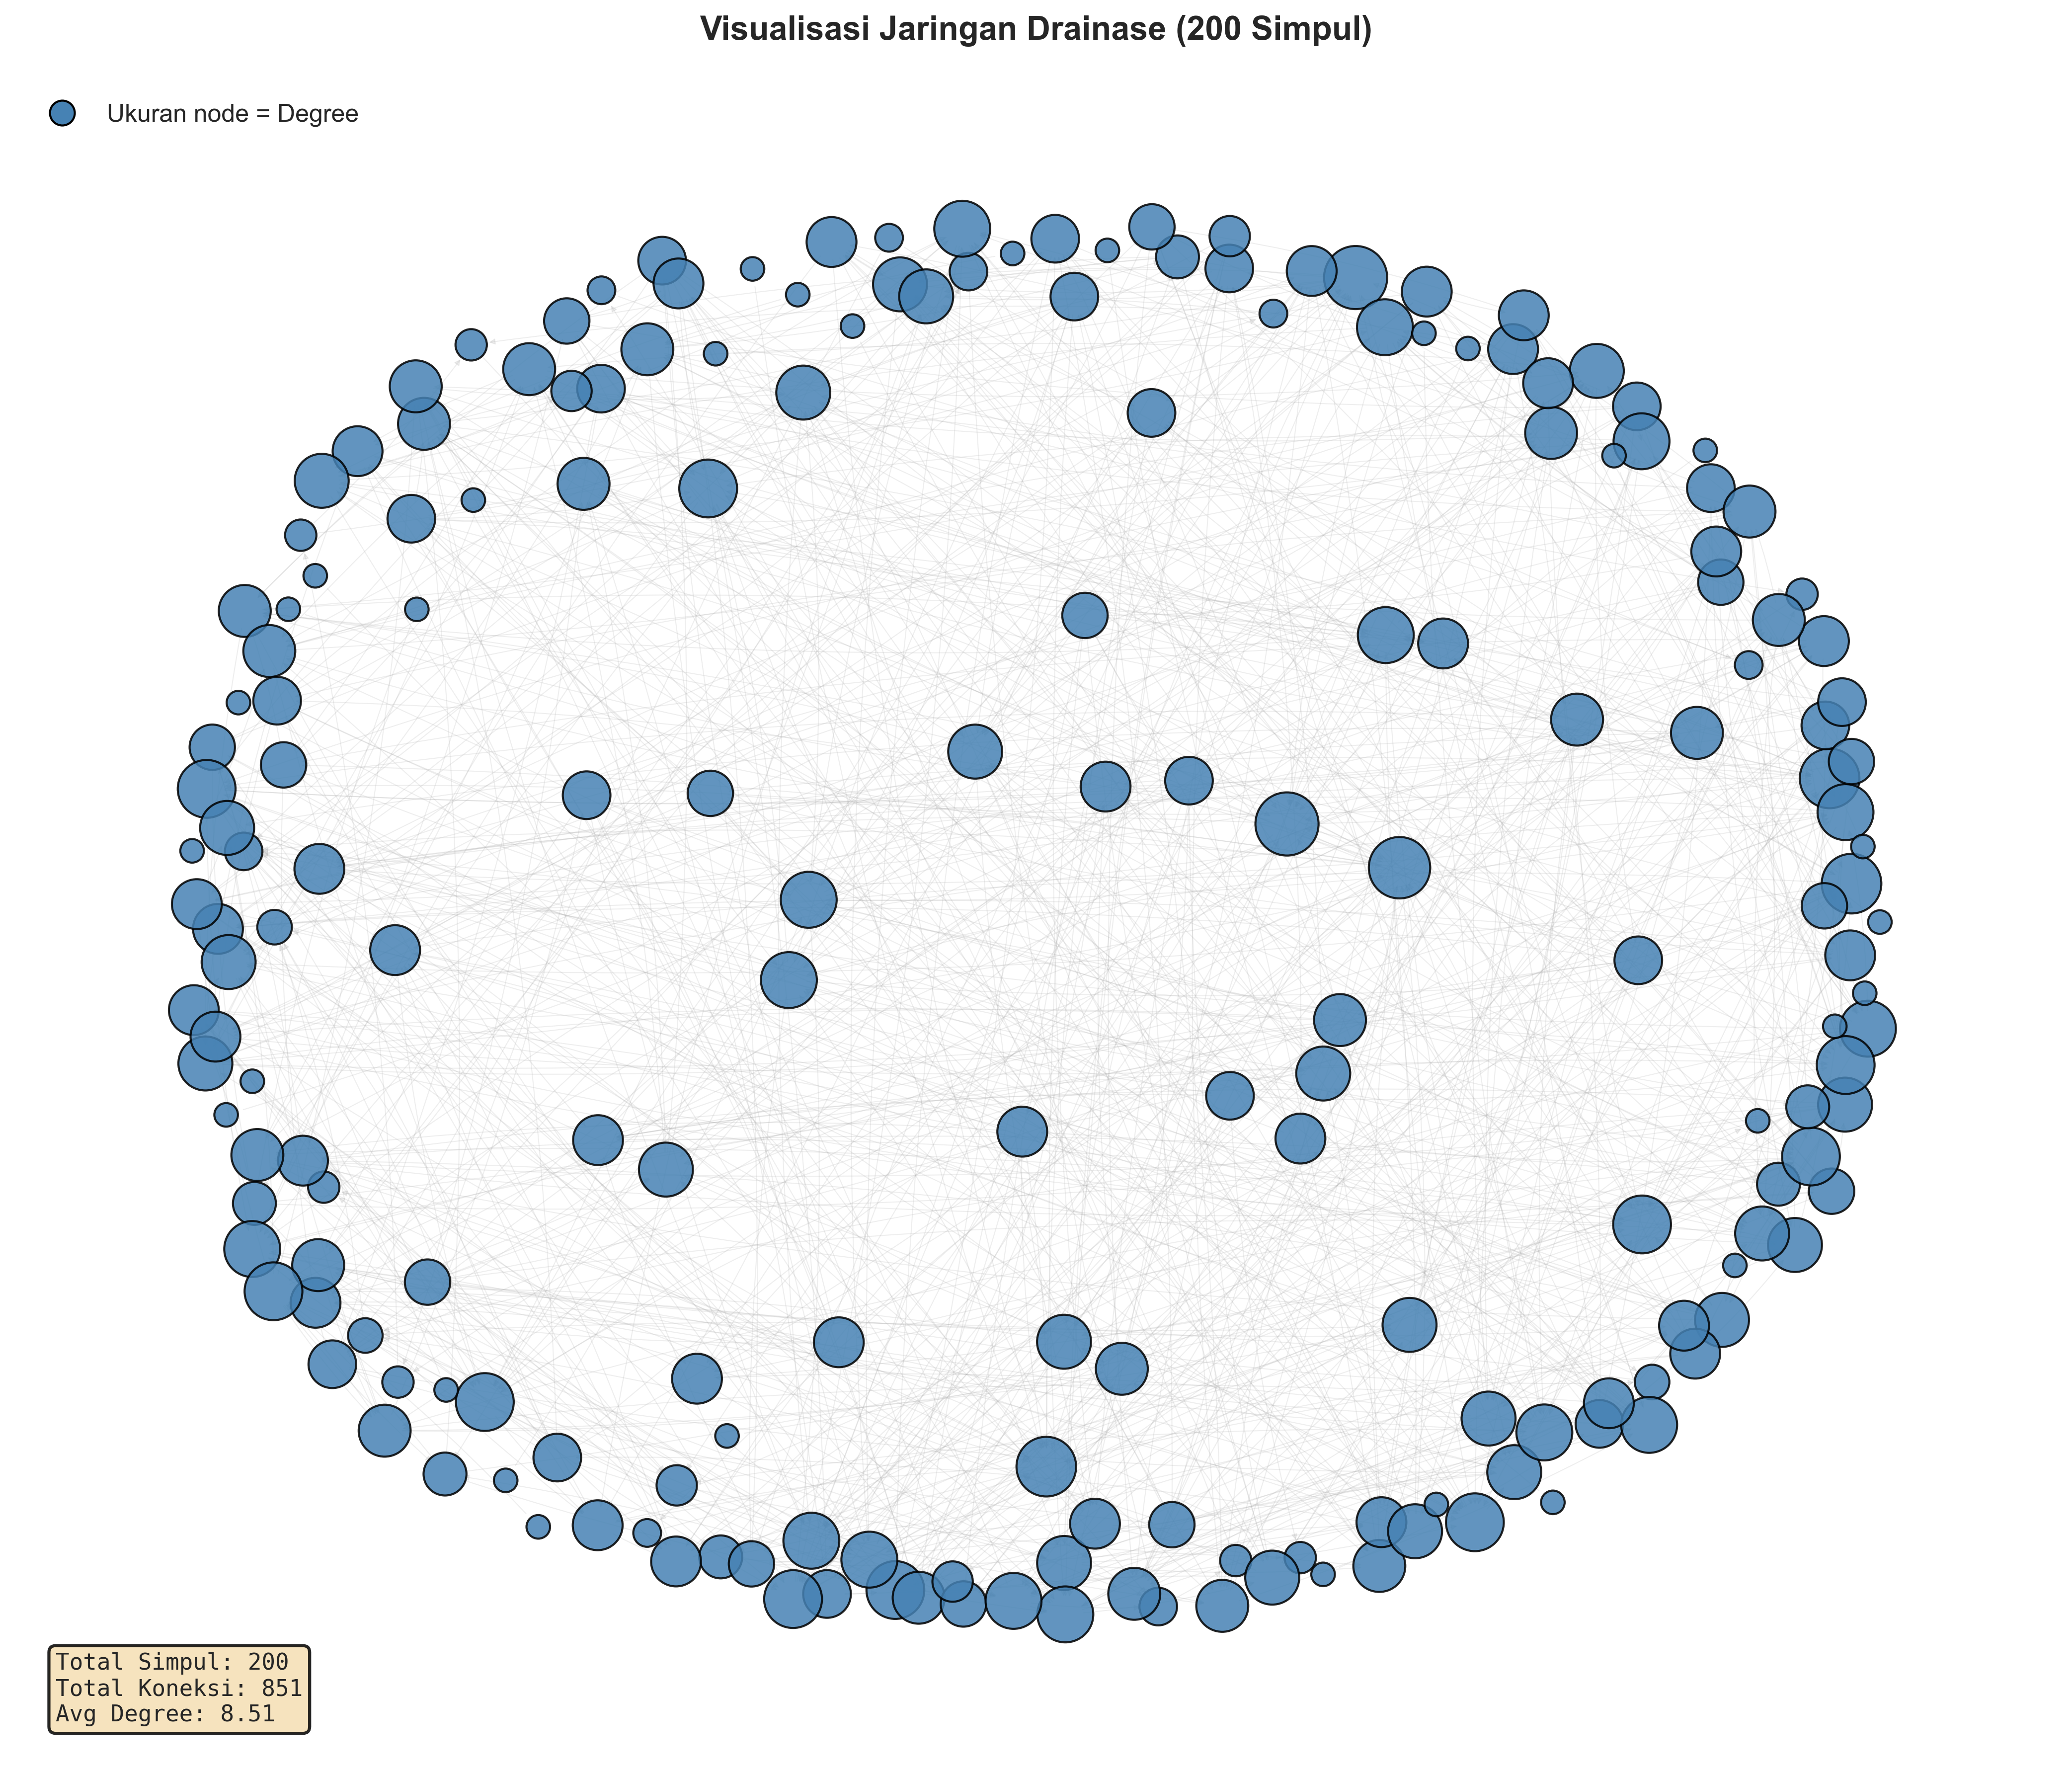
\includegraphics[width=0.85\columnwidth]{Jaringan.png}
\caption{Visualisasi Jaringan Dummy}
\label{fig:jaringan}
\end{figure}

\noindent Gambar \ref{fig:jaringan} menampilkan struktur jaringan dummy dengan 200 simpul dan 851 edges yang digunakan dalam penelitian ini. Visualisasi ini menunjukkan konektivitas antar simpul dalam jaringan drainase yang dimodelkan. Setiap simpul merepresentasikan titik dalam sistem drainase (seperti pertemuan saluran atau titik pembuangan), sedangkan edges merepresentasikan saluran yang menghubungkan antar titik tersebut. Dari visualisasi ini, kita bisa melihat bahwa jaringan memiliki struktur yang cukup kompleks dengan beberapa simpul yang memiliki konektivitas tinggi (banyak terhubung ke simpul lain) dan beberapa simpul yang berada di pinggiran jaringan.

\subsection{Implementasi Algoritma}

Implementasi dilakukan menggunakan Python 3.12 dengan library NumPy untuk komputasi matriks dan Pandas untuk manipulasi data. NumPy dipilih karena library ini menyediakan fungsi-fungsi khusus untuk komputasi aljabar linier yang sangat efisien, terutama \texttt{numpy.linalg.eigh()} untuk menghitung nilai eigen dan vektor eigen dari matriks simetris. Berikut snippet kode utama yang digunakan:

\begin{lstlisting}[language=Python]
import numpy as np
import pandas as pd

class HydraulicDrainageAnalyzer:
    def construct_matrices(self):
        # Symmetric adjacency matrix
        A = np.zeros((n, n))
        for edge in edges:
            A[edge.src, edge.tgt] = 1
            A[edge.tgt, edge.src] = 1

        # Laplacian: L = D - A
        D = np.diag(A.sum(axis=1))
        L = D - A
        return L

    def spectral_analysis(self):
        # Eigenvalue decomposition
        vals, vecs = np.linalg.eigh(L)
        lambda2 = vals[1]
        rho_A = np.max(np.abs(np.linalg.eigvalsh(A)))
        return lambda2, rho_A

    def power_iteration(self, max_iter=100, tol=1e-6):
        x = np.random.rand(n)
        for k in range(max_iter):
            x_new = A @ x / np.linalg.norm(A @ x)
            if np.linalg.norm(x_new - x) < tol:
                break
            x = x_new
        return x

    def hydraulic_vulnerability(self, h, Q, R, r_sed):
        # Normalisasi terbalik elevasi
        r_elev = 1.0 - (h - h.min()) / (h.max() - h.min())
        # Rasio hujan terhadap kapasitas
        r_cap = np.clip(R / (Q * 10), 0, 1)
        # Kombinasi berbobot
        H_vul = (0.25*r_elev + 0.30*r_cap 
                 + 0.25*r_sed + 0.20*r_load)
        return H_vul

    def integrated_vulnerability(self):
        Vul = 0.30 * c + 0.30 * deg / (n - 1) + 0.40 * H_vul
        Vul = np.power(Vul, 0.7) * (0.95 / Vul.max())
        return Vul
\end{lstlisting}

Kode lengkap tersedia di repository bersama dataset.

\subsection{Hasil Analisis Spektral}

Hasil dekomposisi eigen pada matriks Laplacian menghasilkan spektrum eigenvalue dengan properti seperti yang ditunjukkan Tabel~\ref{tab:spektral} berikut.

\begin{table}[!htbp]
\centering
\caption{Properti Spektral Jaringan}
\label{tab:spektral}
\begin{tabular}{lc}
\toprule
\textbf{Metrik} & \textbf{Nilai} \\
\midrule
Algebraic connectivity ($\lambda_2$) & 0.0749 \\
Spectral radius ($\rho(A)$) & 10.23 \\
Average degree & 7.89 \\
Degree range & 1--16 \\
$\rho(A)/\text{deg}_{\text{avg}}$ & 1.30 \\
\bottomrule
\end{tabular}
\end{table}

Nilai $\lambda_2 = 0.0749 < 0.1$ mengindikasikan jaringan sangat rentan terhadap fragmentasi. Untuk memahami apa artinya: algebraic connectivity $\lambda_2$ adalah nilai eigen kedua terkecil dari matriks Laplacian yang mengukur seberapa kuat jaringan terhubung. Nilai yang mendekati 0 menunjukkan jaringan mudah "terpisah" menjadi komponen-komponen yang tidak terhubung jika ada simpul kritis yang gagal. Sebagai perbandingan, jaringan yang robust biasanya memiliki $\lambda_2 > 0.1$. Ini sesuai dengan literatur yang menyatakan bahwa nilai $\lambda_2$ kecil berarti konektivitas lemah. Spectral radius $\rho(A) = 10.23$ dengan rasio 1.30 terhadap average degree menunjukkan moderate hub dominance—tidak terlalu ekstrem seperti star topology.

\subsection{Distribusi Kerentanan}

Klasifikasi kerentanan berdasarkan persentil $P_{70}$ dan $P_{30}$ menghasilkan distribusi seperti di Tabel~\ref{tab:distribusi} berikut.

\begin{table}[!htbp]
\centering
\caption{Distribusi Kategori Kerentanan}
\label{tab:distribusi}
\begin{tabular}{lcc}
\toprule
\textbf{Kategori} & \textbf{Jumlah} & \textbf{Persentase} \\
\midrule
High (Vul $\geq$ 0.739) & 60 & 30.0\% \\
Medium (0.615--0.739) & 80 & 40.0\% \\
Low (Vul $\leq$ 0.615) & 60 & 30.0\% \\
\bottomrule
\end{tabular}
\end{table}

Distribusi dengan pola 30-40-30 menunjukkan hasil yang cukup realistis tanpa bias ekstrem. Artinya, dari 200 simpul dalam jaringan, 60 simpul (30\%) termasuk kategori kerentanan tinggi yang perlu perhatian prioritas, 80 simpul (40\%) kategori sedang, dan 60 simpul (30\%) kategori rendah. Standar deviasi 0.143 dan IQR (Interquartile Range) 0.160 mengindikasikan variance memadai --- tidak terlalu seragam namun juga tidak terlalu ekstrem, yang menunjukkan model menghasilkan diferensiasi yang bermakna antar simpul.

\begin{figure}[!htbp]
\centering
\includegraphics[width=\columnwidth]{Kerentanan.png}
\caption{Ranking 15 Simpul Paling Kritis Berdasarkan Skor Kerentanan}
\label{fig:kerentanan}
\end{figure}

\noindent Gambar \ref{fig:kerentanan} menampilkan ranking 15 simpul dengan tingkat kerentanan tertinggi dalam jaringan drainase. Node 94 dengan skor 0.950 merupakan simpul paling kritis, diikuti oleh Node 105 (0.945) dan Node 85 (0.935).

\subsection{Identifikasi Simpul Kritis}

Tabel~\ref{tab:top10} menampilkan 10 simpul dengan tingkat kerentanan tertinggi. Node 94 dengan degree 16 (tertinggi dalam seluruh jaringan) dan eigenvalue centrality 1.0 adalah bottleneck utama yang sangat berpengaruh --- jika simpul ini gagal, dampaknya akan terasa ke banyak bagian jaringan. Seluruh simpul dalam top 10 adalah secondary channels dengan kombinasi high degree (rata-rata 13.1 dibandingkan 7.89 untuk seluruh jaringan) dan risiko hidraulik yang signifikan. Parameter E-C (Eigenvalue Centrality) menunjukkan seberapa "sentral" simpul dalam struktur jaringan, D-C (Degree Centrality) menunjukkan proporsi koneksi simpul, sedangkan H-V (Hydraulic Vulnerability) menggabungkan faktor fisik seperti elevasi, kapasitas, dan beban aliran.

\begin{table}[!htbp]
\centering
\caption{Top 10 Simpul Kritis dengan Parameter Lengkap}
\label{tab:top10}
\scriptsize
\begin{tabular}{@{}ccccccccc@{}}
\toprule
\textbf{Node} & \textbf{Deg} & \textbf{Vul} & \textbf{E-C} & \textbf{D-C} & \textbf{H-V} & \textbf{Elev} & \textbf{Cap} & \textbf{Rain} \\
\midrule
94 & 16 & 0.950 & 1.000 & 0.080 & 0.592 & 13.5 & 3.5 & 52.2 \\
105 & 12 & 0.945 & 0.833 & 0.060 & 0.721 & 12.9 & 2.8 & 66.2 \\
85 & 14 & 0.935 & 0.883 & 0.070 & 0.656 & 12.2 & 3.1 & 55.0 \\
109 & 14 & 0.924 & 0.933 & 0.070 & 0.595 & 13.2 & 3.9 & 51.9 \\
115 & 11 & 0.903 & 0.559 & 0.055 & 0.843 & 9.2 & 3.0 & 44.3 \\
122 & 14 & 0.897 & 0.746 & 0.070 & 0.678 & 15.0 & 4.6 & 77.4 \\
114 & 11 & 0.885 & 0.600 & 0.055 & 0.776 & 10.5 & 3.1 & 67.5 \\
108 & 12 & 0.874 & 0.699 & 0.060 & 0.675 & 15.2 & 4.3 & 86.9 \\
111 & 15 & 0.865 & 0.712 & 0.075 & 0.636 & 14.2 & 4.2 & 57.2 \\
140 & 12 & 0.865 & 0.687 & 0.060 & 0.665 & 13.2 & 4.6 & 62.4 \\
\bottomrule
\end{tabular}
\bigskip
\vspace{2pt}
\centering
\scriptsize\textit{E-C=Eigen-C, D-C=Deg-C, H-V=H-Vul, Elev=Elev(m), Cap=Cap(m³/s), Rain=Rain(mm/h)}
\end{table}

\subsection{Validasi Teoritis}

Tabel~\ref{tab:validation} menunjukkan hasil validasi terhadap 7 kriteria teoritis. Perlu ditekankan bahwa validasi ini bersifat \textit{consistency check} terhadap ekspektasi teoritis dan konsistensi internal model, bukan validasi empiris terhadap data lapangan riil. Semua korelasi sesuai ekspektasi teoritis dan punya signifikansi statistik tinggi ($p < 0.001$), mengonfirmasi validitas pendekatan yang digunakan.

\begin{table}[!htbp]
\centering
\caption{Hasil Validasi Multi-Kriteria}
\label{tab:validation}
\small
\begin{tabular}{lcc}
\toprule
\textbf{Test} & \textbf{Hasil} & \textbf{Status} \\
\midrule
Degree $\to$ Vul (positive) & $r=0.400$ & \checkmark \\
Elevation $\to$ Vul (negative) & $r=-0.316$ & \checkmark \\
Sediment $\to$ Vul (positive) & $r=0.509$ & \checkmark \\
Hydraulic Load $\to$ Vul (positive) & $r=0.562$ & \checkmark \\
Eigen-C $\to$ Vul (positive) & $r=0.715$ & \checkmark \\
Multi-factor balance & 5/10 deg, 8/10 hyd & \checkmark \\
Distribution ($\sigma$, IQR) & 0.143, 0.160 & \checkmark \\
\midrule
\textbf{Overall Score} & \textbf{7/7 (100\%)} & \checkmark \\
\bottomrule
\end{tabular}
\end{table}

Semua kriteria validasi menunjukkan hasil yang sesuai dengan ekspektasi teoritis. Korelasi positif antara \textit{degree} dan kerentanan ($r=0.400$) masuk akal karena simpul dengan banyak koneksi memiliki peran lebih penting dalam jaringan --- jika simpul ini bermasalah, dampaknya akan menyebar ke banyak bagian lain. Korelasi negatif antara elevasi dan kerentanan ($r=-0.316$) juga logis: simpul di elevasi lebih tinggi cenderung tidak tergenang saat banjir, sehingga lebih aman. Sebaliknya, korelasi positif untuk sedimen ($r=0.509$) dan beban hidraulik ($r=0.562$) menunjukkan bahwa simpul dengan akumulasi sedimen tinggi atau pemanfaatan kapasitas tinggi lebih rentan terhadap kegagalan sistem. Eigenvalue centrality yang berkorelasi positif dengan kerentanan ($r=0.715$) --- korelasi terkuat --- memvalidasi bahwa power iteration method memang menangkap informasi penting tentang struktur jaringan yang relevan dengan analisis risiko drainase.

\subsection{Interpretasi Hasil}

\subsubsection{Catatan tentang Representasi Tak-Berarah}
Hasil analisis perlu diinterpretasikan dengan memahami bahwa representasi tak-berarah memberikan penilaian kerentanan yang bersifat \textit{konservatif}: simpul yang teridentifikasi kritis adalah simpul yang penting untuk konektivitas struktural jaringan. Dalam sistem drainase riil yang berarah, simpul-simpul ini tetap kritis, dengan tambahan kemungkinan ada simpul upstream tertentu yang kritikalitasnya lebih tinggi karena efek cascade downstream. Dengan demikian, hasil ini dapat digunakan sebagai \textit{lower bound} untuk identifikasi simpul kritis---prioritas pemeliharaan yang dihasilkan valid dan aman, meskipun analisis berarah lebih lanjut dapat mengungkap prioritas tambahan.

\subsubsection{Kerentanan Jaringan}
Nilai $\lambda_2 = 0.075$ jauh di bawah threshold 0.1, menandakan jaringan sangat rentan terhadap pemisahan. Kalau satu simpul kritis rusak, jaringan bisa terpecah jadi komponen terpisah.

\subsubsection{Dominasi Hub}
Moderate spectral radius ($\rho(A)/\text{deg}_{\text{avg}} = 1.30$) menunjukkan distribusi beban relatif merata dengan beberapa hub strategis. Tidak terlalu ekstrem seperti star network.

\subsubsection{Integrasi Hidraulik}
Top 10 nodes menunjukkan kombinasi high degree (topological importance) dan risiko hidraulik yang tinggi. Node 115 dengan degree 11 (moderate) namun H-vul 0.843 (tertinggi) membuktikan faktor hidraulik memberikan kontribusi signifikan, bukan hanya aspek topologi semata.

\subsubsection{Rekomendasi Praktis}
Prioritas penanganan:
\begin{enumerate}
    \item Node 94, 105, 85: Hub kritis dengan high degree
    \item Node 115, 114: Risiko hidraulik tinggi (sediment, elevasi rendah)
    \item 60 nodes (30\%) kategori high: Fokus maintenance
\end{enumerate}



\section{KESIMPULAN}
Penelitian ini berhasil menerapkan pendekatan analisis spektral berbasis eigenvalue decomposition dan power iteration method untuk mengidentifikasi titik-titik kritis dalam jaringan drainase perkotaan. Melalui integrasi antara analisis topologi jaringan dan parameter hidraulik, penulis mengembangkan metode penilaian kerentanan yang lebih komprehensif dibandingkan pendekatan konvensional yang hanya mengevaluasi komponen secara terpisah.

Hasil analisis menunjukkan bahwa nilai algebraic connectivity sebesar $\lambda_2 = 0.075$ mengindikasikan jaringan dummy yang dianalisis memiliki tingkat kerentanan yang cukup tinggi terhadap fragmentasi. Artinya, jika terdapat kegagalan pada simpul-simpul kritis, jaringan bisa terpecah menjadi beberapa komponen terpisah yang tidak terhubung, sehingga fungsi drainase menjadi tidak optimal. Korelasi yang kuat antara eigenvalue centrality dan skor kerentanan ($r=0.715$) membuktikan bahwa pendekatan spektral mampu menangkap informasi struktural penting yang tidak terlihat dari analisis konektivitas lokal saja. Selain itu, integrasi faktor hidraulik seperti risiko sedimentasi ($r=0.509$) dan beban hidraulik ($r=0.562$) memberikan kontribusi signifikan dalam menghasilkan penilaian kerentanan yang lebih realistis dan aplikatif.

Distribusi kerentanan yang dihasilkan menunjukkan pola 30-40-30, dengan sekitar 60 simpul (30\%) masuk dalam kategori kerentanan tinggi yang memerlukan prioritas pemeliharaan tertinggi. Analisis sensitivitas bobot membuktikan bahwa model cukup robust terhadap variasi parameter moderat, dengan kestabilan ranking tertinggi pada konfigurasi bobot baseline. Metode ini menghasilkan ranking kuantitatif yang dapat langsung digunakan untuk perencanaan pemeliharaan preventif dan alokasi sumber daya secara lebih efisien.

Meskipun penelitian ini memberikan kontribusi metodologis yang signifikan, terdapat beberapa keterbatasan yang perlu diperhatikan dan dapat menjadi arah pengembangan selanjutnya. Pertama, penggunaan representasi graf tak-berarah mengorbankan informasi tentang dependensi asimetris dalam aliran drainase (upstream-downstream relationship). Meskipun simplifikasi ini valid untuk analisis first-order structural vulnerability dan konsisten dengan praktik umum dalam network science \cite{b6, b7}, analisis yang lebih komprehensif dapat menggunakan directed graph dengan metode seperti PageRank centrality atau directed Laplacian untuk menangkap efek cascade downstream. Kedua, model yang dikembangkan bersifat \textit{statis} --- menganalisis snapshot jaringan pada satu waktu tertentu tanpa mempertimbangkan dinamika temporal. Padahal, sistem drainase sangat dipengaruhi oleh faktor waktu: risiko sedimentasi bertambah secara bertahap seiring waktu, beban hidraulik berfluktuasi drastis dalam hitungan jam saat hujan ekstrem, dan kondisi struktural infrastruktur mengalami degradasi seiring usia. Pengembangan model \textit{dinamis} yang memasukkan variabel waktu atau skenario temporal (misalnya skenario curah hujan 5 tahunan vs 50 tahunan, atau analisis time-series degradasi infrastruktur) akan memberikan insight yang jauh lebih mendalam dan aplikatif untuk perencanaan jangka panjang.

Kedua, penelitian ini masih menggunakan data dummy karena keterbatasan akses terhadap data infrastruktur publik yang lengkap. Validasi dengan data riil dari sistem drainase kota aktual (misalnya satu kecamatan di Jakarta atau Bandung) sangat diperlukan untuk memverifikasi akurasi prediksi dan mengungkap anomali yang mungkin tidak terdeteksi pada data simulasi. Ketiga, perbandingan dengan metrik sentralitas lain seperti \textit{betweenness centrality} atau \textit{closeness centrality} dapat memberikan perspektif tambahan tentang keunggulan metode spektral. Dengan demikian, pendekatan analisis spektral terintegrasi ini berhasil memberikan perspektif sistemik terhadap integritas jaringan drainase dan dapat menjadi fondasi untuk pengembangan sistem monitoring dan early warning berbasis waktu nyata di masa mendatang.



\section{UCAPAN TERIMA KASIH}
Penulis mengucapkan syukur kepada Allah SWT atas segala rahmat dan karunia-Nya sehingga makalah ini dapat diselesaikan dengan baik. Ucapan terima kasih juga disampaikan kepada Mr. Rila Mandala dan tim pengajar IF2123 Aljabar Linear dan Geometri yang telah memberikan fondasi teoritis yang kuat dalam bidang aljabar linear. Apresiasi juga disampaikan kepada rekan-rekan mahasiswa Teknik Informatika ITB atas diskusi dan masukan konstruktif yang sangat membantu selama penulisan makalah ini.



\begin{thebibliography}{00}
\bibitem{b1} F.R.K. Chung, ``Spectral Graph Theory,'' American Mathematical Society, Providence, RI, 1997. Diakses: 11 Desember 2025.

\bibitem{b2} M. Fiedler, ``Algebraic connectivity of graphs,'' Czechoslovak Mathematical Journal, vol. 23, no. 2, pp. 298-305, 1973. Diakses: 11 Desember 2025.

\bibitem{b3} U. Von Luxburg, ``A tutorial on spectral clustering,'' Statistics and Computing, vol. 17, no. 4, pp. 395-416, 2007. Diakses: 12 Desember 2025.

\bibitem{b4} P. Bonacich, ``Power and centrality: A family of measures,'' American Journal of Sociology, vol. 92, no. 5, pp. 1170-1182, 1987. Diakses: 12 Desember 2025.

\bibitem{b5} G. H. Golub and C. F. Van Loan, ``Matrix Computations,'' 3rd ed., Johns Hopkins University Press, Baltimore, 1996. Diakses: 11 Desember 2025.

\bibitem{b6} M.E.J. Newman, ``Networks: An Introduction,'' Oxford University Press, Oxford, 2010. Diakses: 23 Desember 2025.

\bibitem{b7} A.-L. Barabási, ``Network Science,'' Cambridge University Press, Cambridge, 2016. Diakses: 23 Desember 2025.

\bibitem{b8} L. W. Mays, ``Urban Water Supply Management Tools,'' McGraw-Hill, New York, 2000. Diakses: 24 Desember 2025.

\bibitem{b9} R. Munir, ``Aljabar Linear dan Geometri,'' Informatika, Bandung, 2024. Diakses: 12 Desember 2025.

\bibitem{b10} L. D. F. Costa et al., ``Characterization of complex networks: A survey of measurements,'' Advances in Physics, vol. 56, no. 1, pp. 167-242, 2007. Diakses: 23 Desember 2025.
\end{thebibliography}



\section*{Lampiran Program dan Video}
\begin{enumerate}
    \item \texttt{https://github.com/Akram17t/MakalahALGEO/}
\end{enumerate}

\vspace{3em}
\section*{Pernyataan}
Dengan ini saya menyatakan bahwa makalah yang saya tulis ini adalah tulisan saya sendiri, bukan saduran, atau terjemahan dari makalah orang lain, dan bukan plagiat.

\vspace{2em}
\begin{flushright}
Jakarta, 24 Desember 2025

\vspace{1em}

\includegraphics[width=4cm]{TTD.png}\\
\vspace{0.5em}
Nashiruddin Akram, 13524090
\end{flushright}

\end{document}
